\section{Sistemas de inducción de reglas}

\subsection{Algoritmo RIPPER}
El algoritmo RIPPER (Repeated Incremental Pruning to Produce Error Reduction) es una versión mejorada del algoritmo IREP que busca minimizar el error, es decir se intenta reducir el número de ejemplos clasificados incorrectamente \cite{A4}. 

Está diseñado para generar reglas a partir de un conjunto de datos de forma incremental de la siguiente forma, para casos como el estudiado, con múltiples clases \{$ \text{C}_{\text{1}}$, $ \text{C}_{\text{2}}$, $ \text{C}_{\text{3}}$ ... $ \text{C}_{\text{k}}$\}, lo primero es ordenar las clases  de menor a mayor relevancia para intentar extraer reglas que separen la clase con menor relevancia ($ \text{C}_{\text{1}}$) del resto haciendo una llamada al algoritmo IREP siendo $ \text{C}_{\text{1}}$ la clase positiva y el resto la clase negativa \cite{M1}. 

Una vez se obtienen las reglas, todos las instancias que quedan cubiertas por las reglas obtenidas se eliminan del conjunto de datos y se repite el proceso siendo ahora la clase menos relevante $ \text{C}_{\text{2}}$. Cuando solo queda la clase más relevante se termina el proceso y se determina que esta clase es la clase a asignar por defecto.
\subsection{Creación del conjunto de datos}
Para poder comparar los resultados obtenidos con los resultados de los árboles de decisión hemos utilizado los mismos conjunto de datos en ambos casos.

\subsection{Experimentación}
\subsubsection{Pruebas realizadas}
En esta caso se han utilizado los mismos conjunto de datos y los mismos parámetros de la herramienta Weka que se han utilizado con árboles de decisión con el objetivo de poder comprobar las diferencias en la precisión de ambos algoritmos. Dado que se comprobó anteriormente que la eficiencia de un conjunto de datos booleano era muy inferior a utilizar frecuencia de términos solo se ha utilizado esta última aproximación con este algoritmo.

Los conjuntos de datos empleados son los siguientes:
\vspace{1em}
\begin{center}


\begin{tabular}{|c|c|c|}
\hline 
Experimentos & Número de palabras & Número de noticias \\ 
\hline 
Experimento 1 & 1064 & 2842 \\ 
\hline 
Experimento 2 & 1649 & 4478 \\ 
\hline 
Experimento 3 & 2124 & 5253 \\ 
\hline 
\end{tabular} 
\end{center}
\vspace{1em}
Como algoritmo hemos utilizado JRIP en WEKA con un cross-validation de 10 folds para el experimento uno y 15 folds para los experimentos dos y tres.
\subsubsection{Resultados obtenidos}

Los resultados obtenidos muestran una mejora de la precisión del clasificador obtenido conforme se aumenta el tamaño del conjunto de datos, aunque son sucesivos aumentos del conjunto de datos la mejora es cada vez menor. Las tasas de aciertos obtenidas son las siguientes:
\vspace{1em}
\begin{center}


\begin{tabular}{|c|c|c|c|}
\hline 
- & Experimento 1 & Experimento 2 & Experimento 3 \\ 
\hline 
Tasa de acierto & 61.7171\% & 69.1603\% & 70.2456\% \\ 
\hline 
\end{tabular} 
\end{center}
\vspace{1em}
Las matrices de confusión obtenidas son las siguientes:

Experimento 1
\begin{center}
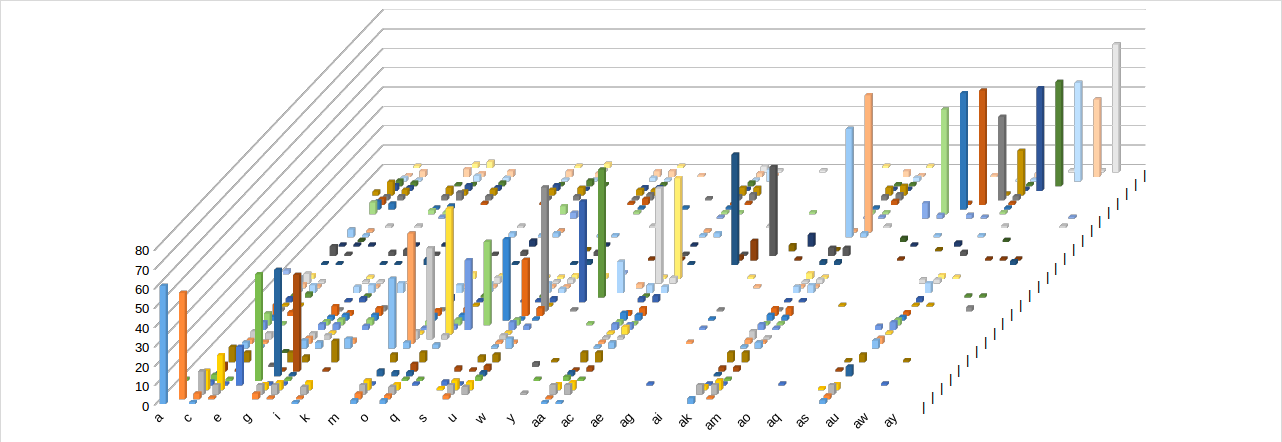
\includegraphics[width=\textwidth]{ripper/RIPPER_80_CV15.png} 
\end{center}
Experimento 2
\begin{center}
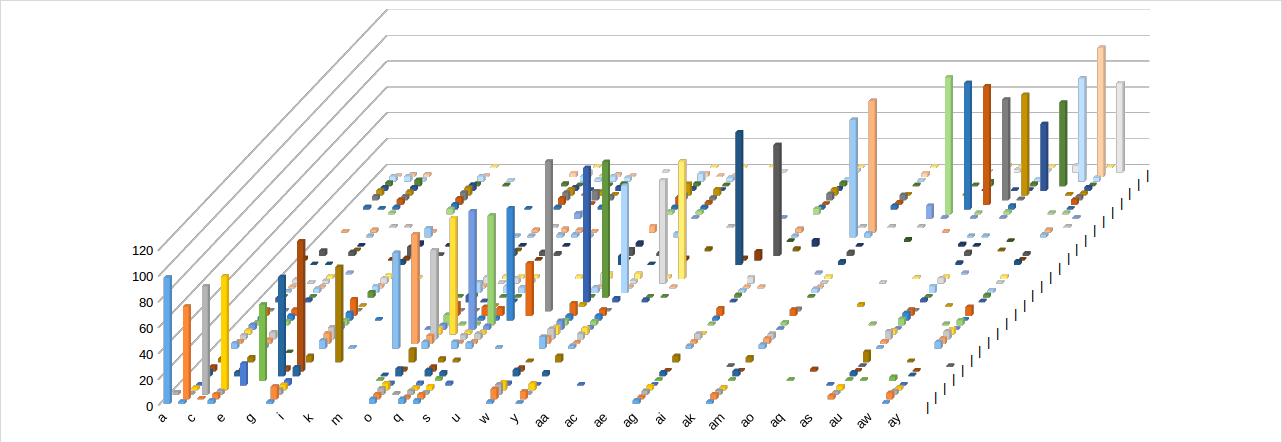
\includegraphics[width=\textwidth]{ripper/RIPPER_125_CV15.png} 
\end{center}
Experimento 3
\begin{center}
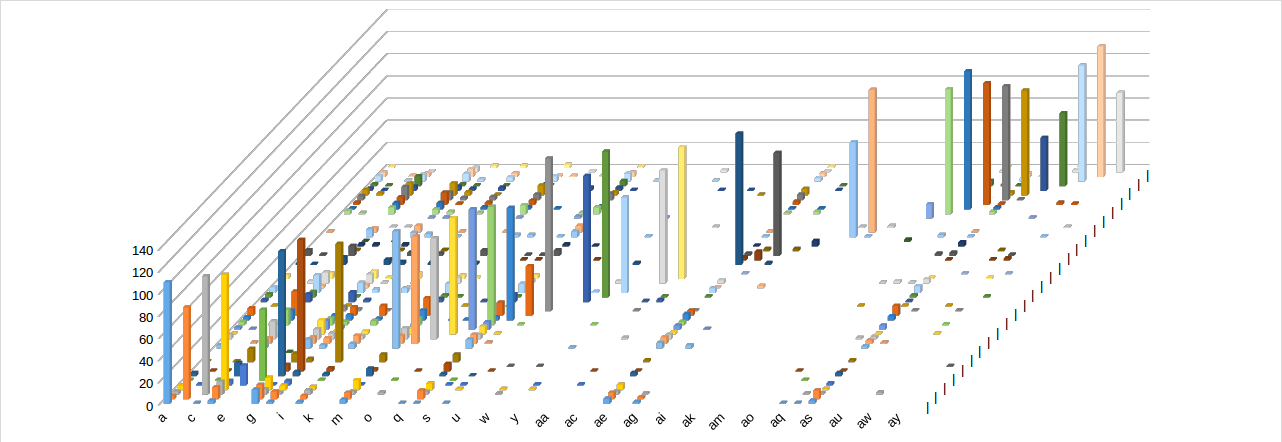
\includegraphics[width=\textwidth]{ripper/RIPPER_175_CV15.png} 
\end{center}

Comparando este algoritmo con los resultados obtenidos en \ref{subsec:resj48}, podemos observar que este algoritmo no presenta problemas con categorías concretas, no presenta problemas con las categorías \textit{Ayuntamiento}, \textit{Cultura} o \textit{Generales}, pero en este caso el error en cada categoría es mayor, de media, el ratio de falsos positivos con RIPPER es mayor que el encontrado con árboles de decisión.
\subsection{Extracción de reglas}

Como en casos anteriores usamos un programa en Java para obtener las reglas en un fichero .clp adaptándolo para poder procesar como entrada las reglas en el formato que tiene Weka.
 



